\documentclass[final]{beamer}
\usetheme{SD}
\usepackage[orientation=landscape,size=custom,width=160,height=90,scale=1.9,debug]{beamerposter}
%\usepackage[absolute,overlay]{textpos}
%\setlength{\TPHorizModule}{1cm}
%\setlength{\TPVertModule}{1cm}

\title{BioConductor:  Open Source Tools for the Analysis and Comprehension of Genomic Data}
\author{Bioconductor Core Development Group}
\footer{More information at \texttt{\url{http://bioconductor.org/}}}
\date{April 17, 2012}

\begin{document}
\begin{frame}[t]
  \begin{columns}[t]
    \begin{column}{0.24\linewidth}
      \begin{block}{What is Bioconductor?}
        Bioconductor provides tools for the analysis and comprehension of high-throughput genomic data. Bioconductor uses the R statistical programming language and is open source and open development. It has two releases each year, 554 software packages, and an active user community. Bioconductor is also available as an Amazon Machine Image (AMI).
      \end{block}
      \begin{block}{Microarray Data Analysis}
        \begin{itemize}
        \item{Import Affymetrix, Illumina, Nimblegen, Agilent, and other platforms}
        \item{Microarray quality assessment, normalization, differential expression}
        \item{Clustering and classification}
        \item{Gene set enrichment and pathway analysis}
        \item{Workflows available for:}
     \begin{itemize}
       \item{Gene expression}
       \item{Exon arrays}
       \item{Copy number}
       \item{SNP}
       \item{Methylation}
     \end{itemize}
        \end{itemize}
      \end{block}
      \begin{block}{Annotation Resources}
        \begin{itemize}
          \item{Use microarray probe, gene, pathway, gene ontology, homology and other annotations} 
          \item{Access GO, KEGG, NCBI, Biomart, UCSC, vendor, and other sources}
        \end{itemize}
        \end{block}
      \begin{block}{Other High-throughput Technologies}
        Ability to import, transform, edit, analyze and visualize:
        \begin{itemize}
          \item{Flow cytometry}
          \item{Mass spec}
          \item{qPCR}
          \item{Cell-based assays}
        \end{itemize}
        \end{block}
        \end{column}
    \begin{column}{0.48\linewidth}
      \begin{block}{Graphical Capabilities of Bioconductor}
        \begin{columns}[t]
          \begin{column}{0.33\linewidth}
            \begin{figure}
              \centering
              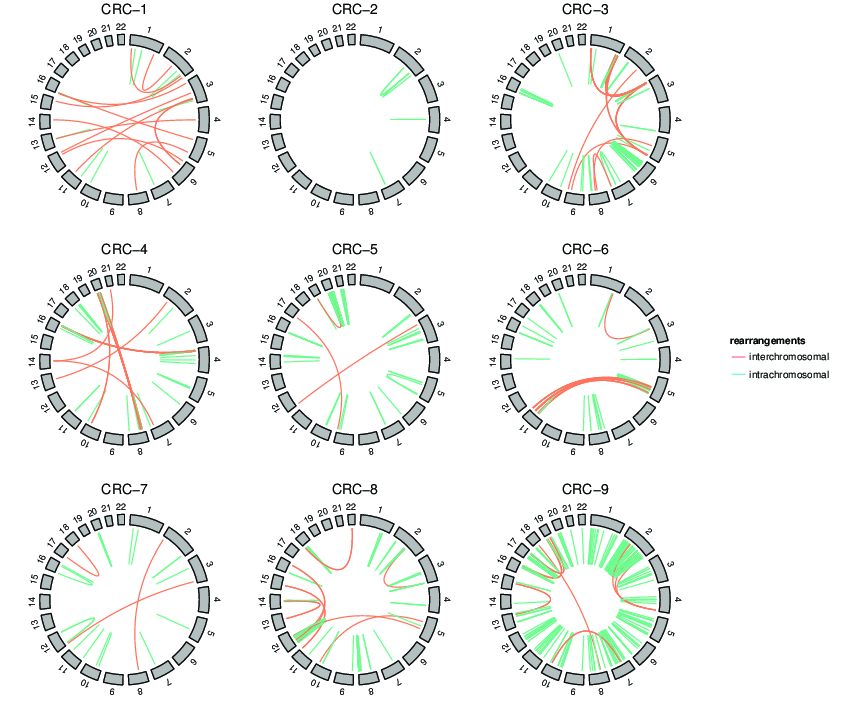
\includegraphics[width=0.85\linewidth]{cir}
              \caption{A circos-like plot from the ggbio package}
            \end{figure}
            \begin{figure}
              \centering
              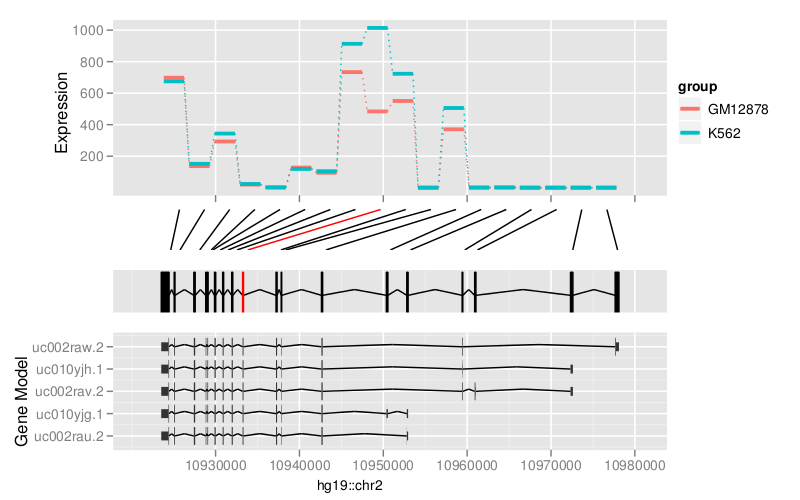
\includegraphics[width=0.85\linewidth]{interval}
              \caption{RNA-seq differential isoform expression from the ggbio package}
            \end{figure}
            \begin{figure}
              \centering
              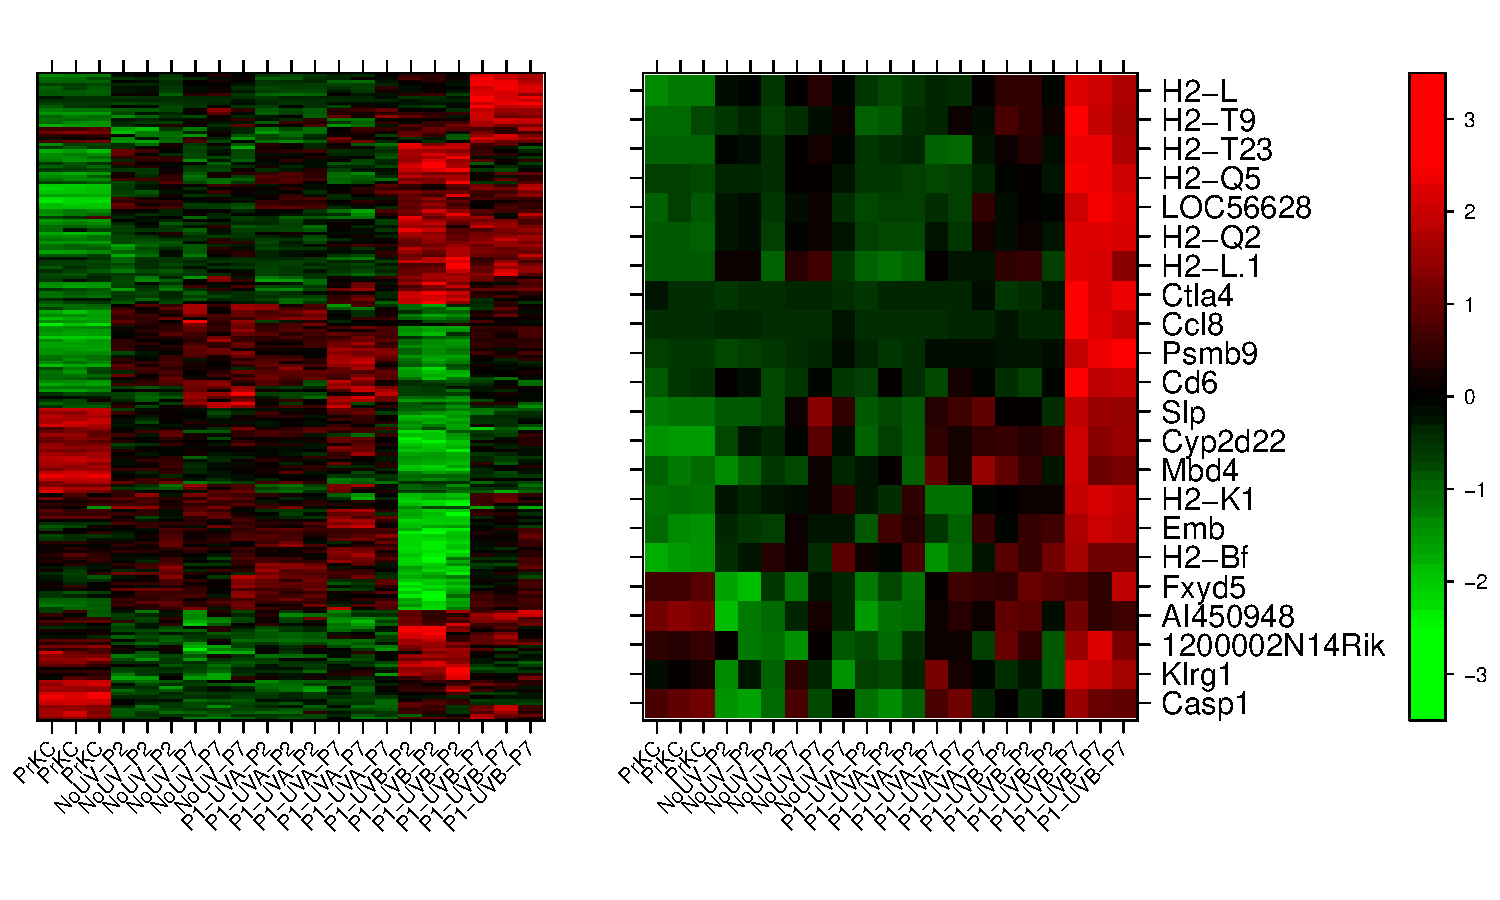
\includegraphics[width=0.85\linewidth]{heatmapPanels}
              \caption{Publication-quality graphics with R}
            \end{figure}
          \end{column}
          \begin{column}{0.33\linewidth}
            \begin{figure}
              \centering
              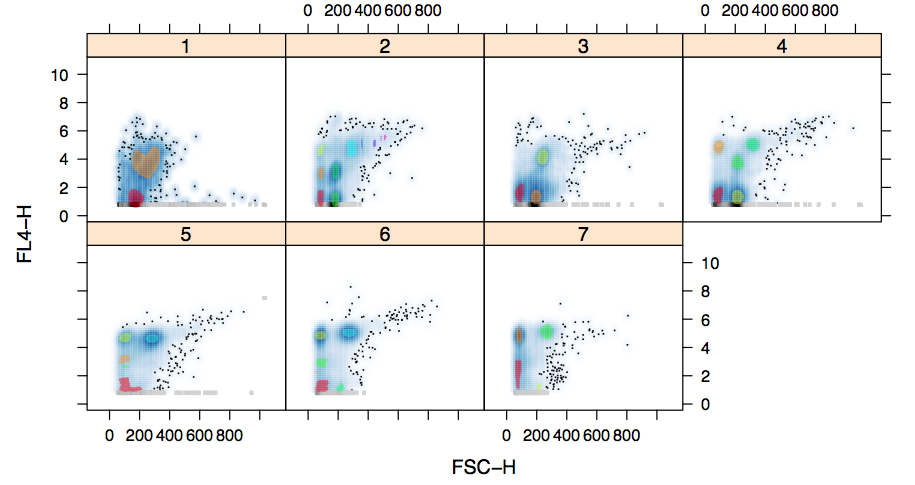
\includegraphics[width=0.85\linewidth]{flowFilter}
              \caption{Flow cytometry filtering and quantification}
            \end{figure}
            \begin{figure}
              \centering
              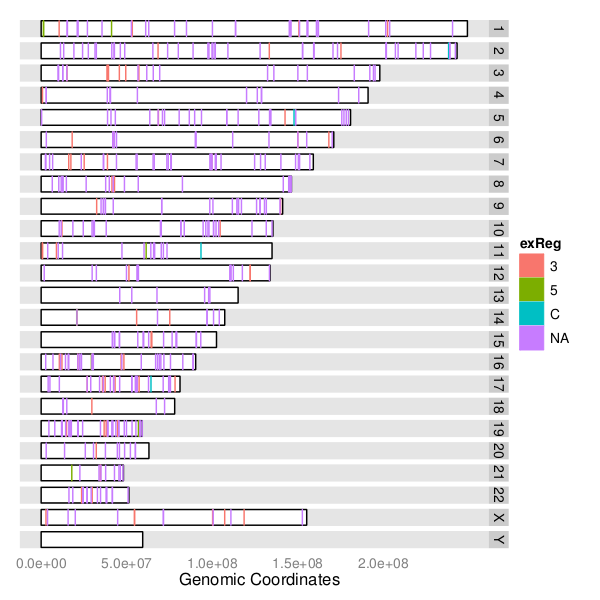
\includegraphics[width=0.85\linewidth]{stacked-darn}
              \caption{Genome overview plot from the ggbio package}
            \end{figure}
            \begin{figure}
              \centering
              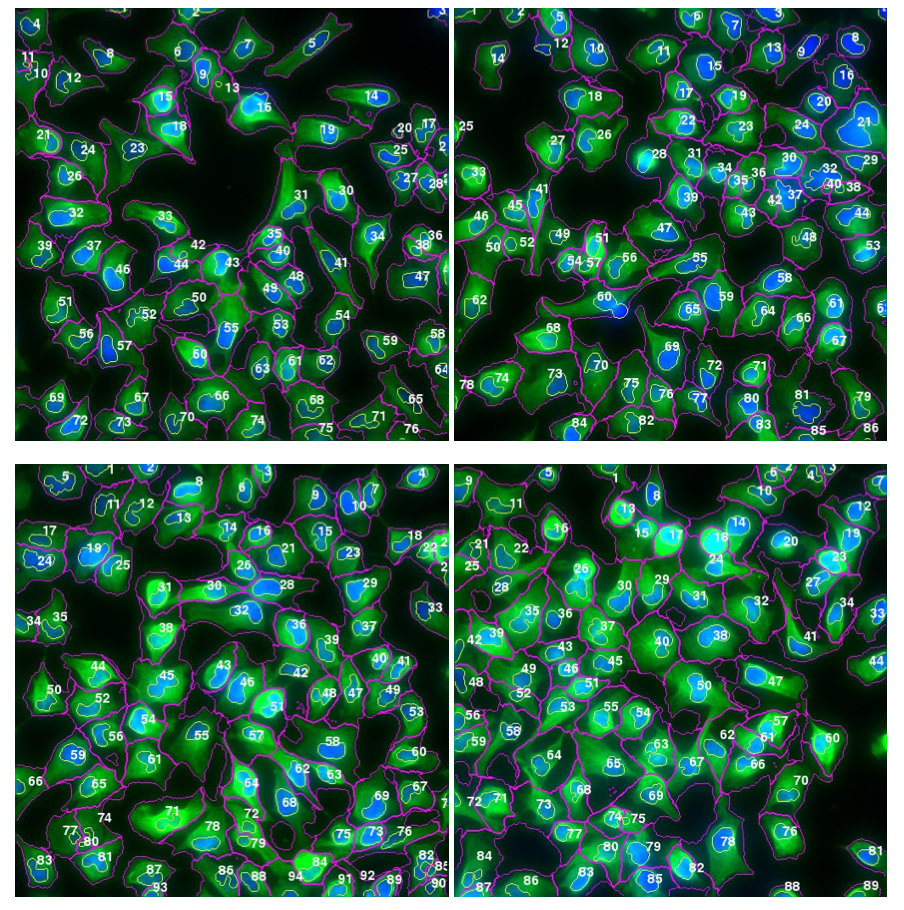
\includegraphics[width=0.85\linewidth]{ebimage}
              \caption{Image segmentation using the EBImage package}
            \end{figure}
          \end{column}
          \begin{column}{0.33\linewidth}
            \begin{figure}
              \centering
              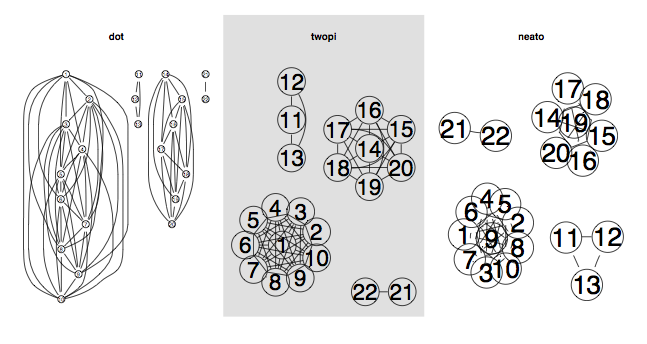
\includegraphics[width=0.85\linewidth]{rgraphviz}
              \caption{Arbitrary graph layout with Rgraphviz}
            \end{figure}
            \begin{figure}
              \centering
              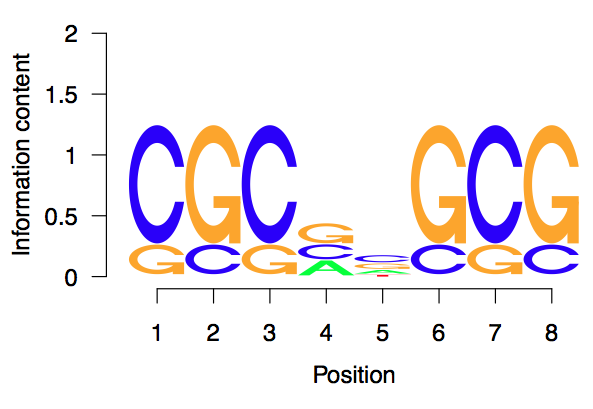
\includegraphics[width=0.85\linewidth]{cosmo}
              \caption{Motif discovery and display with the cosmo package}
            \end{figure}
            \begin{figure}
              \centering
              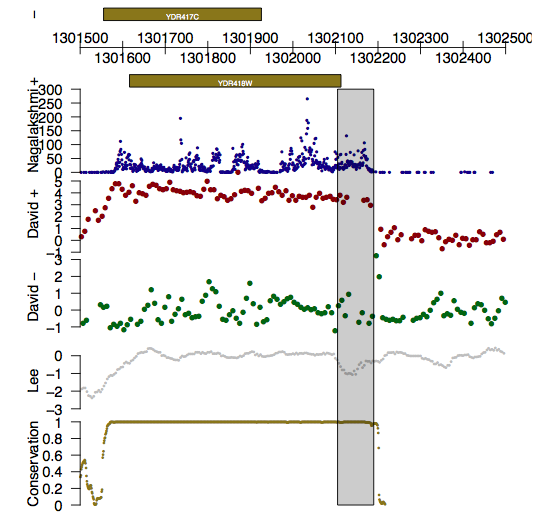
\includegraphics[width=0.85\linewidth]{genomegraphs}
              \caption{Layer data and Ensembl annotation onto figures using GenomeGraphs}
            \end{figure}
          \end{column}
        \end{columns}
      \end{block}

 \end{column}
    \begin{column}{0.24\linewidth}
      \begin{block}{Next-Generation Sequencing Analysis}
        \begin{itemize}
          \item{Import fasta, fastq, ELAND, MAQ, BWA, Bowtie, BAM, gff, bed, wig, and other sequence formats} 
          \item{Trim, transform, align, and manipulate sequences}
          \item{Workflows}
            \begin{itemize}
              \item{Quality assessment}
              \item{ChIP-seq}
              \item{RNA-seq and differential expression}
            \end{itemize}
          \item{Access the NCBI Sequence Read Archive}
        \end{itemize}
      \end{block}
      \begin{block}{Genomic Variants}
        \begin{itemize}
          \item{Read and write VCF files}
          \item{Identify coding variants}
          \item{Use SIFT and PolyPhen to annotate variants}
          \item{Overlap variants with arbitrary genomic annotations}
        \end{itemize}
      \end{block}
      \begin{block}{Data Integration}
        Use of consistent data structures in the R statistical computing environment allows for complex data integration and multi-assay hypothesis generation and testing.
      \end{block}
      \begin{block}{Community, Training, and Education}
\small{Bioconductor runs training and education programs regularly throughout the year all over the world.  The annual Bioconductor Conference is held in Seattle each summer.  The email list is very active and includes discussions of Bioconductor software as well as statistical and informatics questions.  Online training materials are at the Bioconductor website.}
      \end{block}
      \begin{block}{Bioconductor Core Developers}
        \small{Vince Carey (Harvard), Marc Carlson (FHCRC), Sean Davis (NCI), Wolfgang Huber (EMBL), Rafael Irizarry (Johns Hopkins), James MacDonald (Univ Michigan), Martin Morgan (FHCRC), Valerie Obenchain (FHCRC), Paul Shannon (FHCRC), and Dan Tenenbaum (FHCRC)}
      \end{block}
    \end{column}
    \end{columns}
  \end{frame}
\end{document}
